\chapter{Monopolies And The British Experience}

Britain has often taken the lead on commercial affairs ever since the industrial revolution. Since these earliest of times, the philosophy of the British has been one of laissez-faire, that is, non- intervention in the affairs of business by government. The work of Huskisson, Peel and Gladstone can be seen as the deliberate application of these principles to our commercial system.

However it was not just the principle of \textit{laissez-faire} in itself as propounded by Adam Smith and McCulloch that led to a freeing np of the markets from government controL Of as much importance as ideology was the fact that liberalisation favoured the interests of the newly assertive mercantile and manufacturing classes from the time of the 1832 (Parliamentary) Reform Act \citep{Taylor:1972}. This meant that when the problems of monopoly power were highlighted by the railways, the government had no obvious ideological response. Firstly strict regulation, and then public ownership were tried. Both failed and Britain is currently deregulating and privatising in an attempt to regain lost efficiencies. The purpose of this chapter is to examine the results of the attempts to control monopoly power and current policy.

There is a lack of contestability in transport infrastructure owing to the time lags in development: As Sir Alastair Morton, former co-chairman of Eurotunnel put it, \textit{Our generation must invest in the infrastructure for the next two generations} \citep{Morton:1996}. As well as a lack of contestability in terms of new development, there is also the problem of amalgamations removing any current competition, thus creating monopolies. In Britain this was commonplace, \textit{Railway amalgamation is nearly as old as the introduction of steam locomotives on the railways of this country} \citep{Simnett:1923}. This led to abuses of power by the railways' owners in the nineteenth century:

\begin{displayquote}
In a parliamentary speech James Morrisson, MP in 1836 complained that the community was exposed to serious ills from legislature conceding to private companies the powers required for making and working railways, unaccompanied by such conditions as were necessary to secure the public interest \citep{Swift:1995}.
\end{displayquote}
 
Figure \ref{fig:welfare_loss_monopoly} shows how it is possible for a company to abuse monopoly power. In a case of perfect competition, all producers charge a price \textit{p1}, the long run average cost\footnote{As this is a constant, marginal costs and average costs are the same.}, per unit. To charge less than this would lead to bankruptcy, to charge more would lead to customers purchasing the good from a competitor. The supplier will choose to produce units until the cost of production equals the revenue received (AR). This is at quantity \textit{q1}.

In the case of a monopoly, there is no competition and so it is possible to charge more for a good. To obtain maximum profits a supplier would wish to equate the cost of production of the last unit produced (marginal cost) with the revenue that it produces (marginal revenue). This occurs at the lower quantity \textit{q2} at which supply the market will bear a higher cost, \textit{p2}. The extra profit that a monopolist extracts is shaded in the figure. The problem with this situation, is not a political one of wealth redistribution: There is a loss to society in general. The welfare of consumers falls more than the gain taken by the monopolist. The triangle marked on the figure shows the welfare that is lost \citep{Begg:1994}.

\begin{figure}
\tikzstyle{arrow} = [thick,->,>=stealth]
\tikzstyle{arrowd} = [thick,dashed,->,>=stealth]
\centering
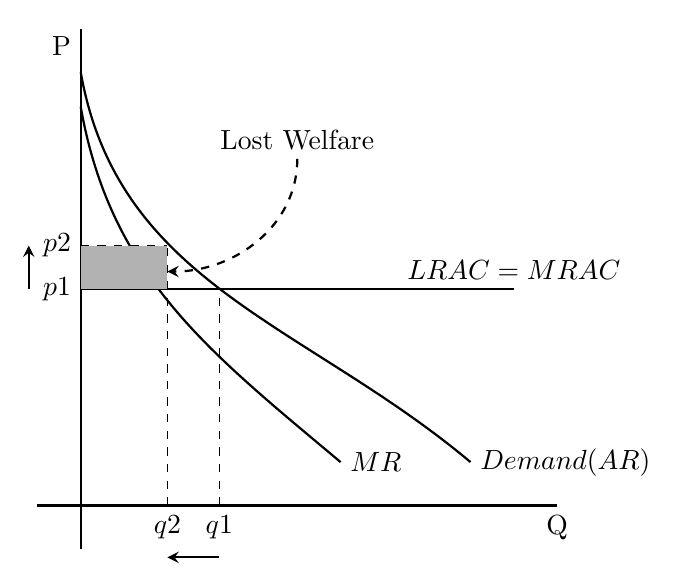
\begin{tikzpicture}[scale=1.1]

% Axis
\draw [thick] (-0.5,-0.0) --(5.5,0);
\draw [thick] (0,-0.5) -- (0,5.5);
\node [left] at (0,5.3) {P};
\node [below] at (5.5,0) {Q};

% Downward slopping line AR
\draw [thick] (0,5) to [out=280,in=140] (4.5,0.5);
\node [right] at (4.5,0.5) {$Demand (AR)$};

% Downward slopping line MR
\draw [thick] (0,4.6) to [out=280,in=140] (3,0.5);
\node [right] at (3,0.5) {$MR$};

% Horizontal Long run cost = marginal cost
\draw [thick] (0,2.5) to (5,2.5);
\node [above] at (5,2.5) {$LRAC=MRAC$};

% Prices and Quantities
\node [left] at (0,3) {$p2$};
\node [left] at (0,2.5) {$p1$};
\node [below] at (1,0) {$q2$};
\node [below] at (1.6,0) {$q1$};

% Price Movement
\draw [dashed](1.6,0)--(1.6,2.5);
\draw [dashed](1,0)--(1,3);
\draw [dashed](0,3)--(1,3);
\draw [arrow](1.6,-0.6) -- (1,-0.6);
\draw [arrow](-0.6,2.5) -- (-0.6,3);

% lost welfare
\node [above] at (2.5,4) {Lost  Welfare};
\draw [arrowd](2.5,4) to [out=270,in=360](1,2.7);
\fill [black!30] (0,3) rectangle (1,2.5);

\end{tikzpicture}
  \caption{Figure showing welfare loss caused by monopoly abuse.}
  \label{fig:welfare_loss_monopoly}
\end{figure}

To control this the Railways Regulation Act of 1844 was passed. It was based on the principle that
\textit{the State should reserve to itself the right to control a possible excessive prosper, it yon the part of the railway companies, and take steps to protect the interests of the public at whose expense such prosperity might he gained.} It outlined two possible powers the government could use: it allowed for the nationalisation of railways companies if needed (that is to say dividends went never ten per cent); There was also the possibility of direct intervention. If a railway company paid a 10\% dividend, or over, the Government was able to revise the company's rates, with the view apparently of bringing earnings below the ten per cent limit \citep{Pratt:1908}.

\begin{displayquote}
By the end of the century, Britain had been left with a railway industry comparable only to mining in the degree of its regulation, yet no less distinguishable from the railway systems of continental Europe by the extent to which construction and management control was still exclusively concentrated in the hands of private enterprise \citep{Taylor:1972}.
\end{displayquote}

There were however advantages to being a regulated industry: it gave the railways the authority to get a job done properly: The Eurostar trip was graphically described by President Mitterrand as \textit{185 mph across northern France, 20 minutes through the tunnel and then time to admire the countryside as you trundle through Kent.} The first part of that trundle, Ashford to Tunbridge, is significantly faster than the second, on into London:

\begin{displayquote}
In 1839 that wonderful early Victorian visionary, Isambard Kingdom BruneI, wrote to a friend who had just been hired to survey a railway from Redhill to Ashford and beyond. BruneI, who was already engaged on creating the Great Western Railway from Paddington to Bristol, said, \textit{Survey it well, my friend, because one day it will link my railway with the Channel Tunnel which must be built.} Her Majesty the Queen, 155 years later, was joined by President Mitterrand in declaring the Channel Tunnel not only build but open for business \citep{Morton:1996}.
\end{displayquote}

Despite the strong regulation of the railways to control monopolistic abuses, the British belief in \textit{laissez-faire}, and thus not controlling economic agents choice of transport mode, has meant that there was no nineteenth century development of an integrated transport plan. Transport modes were left to compete in what was thought a free way: tolled roads competed with tolled railways. However this did not remain so. Tolled roads were disliked by the general populace and it is now the case that bar a few river crossings, all road transport in Britain is free at the point of use. This is one of the reasons that has led to an extraordinary strong favouring of road transport as shown in Table \ref{tab:transport_modes} \citep{DTI:1989}.

A second reason for the choice of road transport is that it allows an individual the freedom to undertake a journey whenever they want to wherever they want. It changes their lifestyle. Historically each change in the level of transport technology has been a facilitator of better lifestyles: the development of Victorian suburbs on the basis of rail or tram which allowed commuting to central city work sites or, more recently the development of large edge-of-town shopping complexes to which the car is often the only form of transport \citep{Benwell:1993}. Not only does a car affect the ability of people to have a better lifestyle, the car itself became an indicator of this better lifestyle, a status symboL Public transport was left to those that could not afford a car \citep{Hibbs:1993a}.

A third reason for the increased use of the car can be traced back to the efforts made by the government in the twenties and thirties to reduce unemployment. The Trunk Road Reconstruction programme launched in 1924 had the explicit purpose increasing spending on roads, thus making them more accessible to the general public, in order to cut the otherwise increasing queues of the jobless \citep{Rodgers:1959}.

\begin{table}[h]
\centering 
\begin{longtable}{lcccc}
\hline
	& \textbf{Road} & \textbf{Rail} & \textbf{Air} & \textbf{Sea}\\ 
\hline
 Very Important & 95 & 8 & 24 & 27 \\
 Fairly Important & 4 & 23 & 34 & 31	\\
 Not Important & 1& 69 & 42 & 42	\\
\hline
\end{longtable}
\caption{Business perceptions of the importance of transport modes}  
\label{tab:transport_modes}
\end{table}


After the Second World War, the British people elected a government with a new ideological bent. It believed that the state should organise all economic activities that bad social repercussions. The railways, having an obvious effect on peoples lives, was bought. Despite the best intentions, this decision was one of the main reasons for the collapse of the public transport sector. From then on, transport and all heavy industry had to fight education, health care and social security for funding in Whitehall. At a moment of belt-tightening. it was obvious which would lose. The Treasury, believing correctly that its mission was to restrict government spending, took the line of least resistance to it. It cut investment.

This continued until 1979 when a new government was elected. It brought with it an absolute belief in the correct working of free markets, and was determined to move back to the traditional British practice of \textit{laissez-faire.} Roads, considered to be the embodiment of individual liberty remained well funded, whilst railways and buses were dispossessed:

\begin{displayquote}
While capital spending on the national road network in 1992 was set at around �2 billion a year, allowing for several major schemes at various locations to be developed, government expenditure on light railway schemes was rationed to �50 million. At that rate only one single line, not a network, can be added to a city every \textit{three} years \citep{Headicar:1994}.
\end{displayquote}

The reminder of this chapter is spent looking at the results of the deregulation of bus services following the 1985 Transport Act and the privatisation of rail services under the 1993 Railways Act. The 1985 Transport Act was a watershed. Previous attempts to deregulate transport had restricted themselves to business and discretionary services. The Transport Act sought to deregulate and subsequently privatise all bus operations outside of London. The purpose was to create a more passenger responsive environment with greater flexibility and innovation in service design and delivery. Research has subsequently shown, however, that many bus operators were risk averse, preferring not to offer strong competition. Within a few years, this became more obvious as nationally based holding companies started buying up many of the smaller operations \citep{Benwell:1993}.

An analysis of services finds a mixed appraisal. In some ways services have improved, with greater use of minibuses serving more bus stops nearer users. In metropolitan areas, between 56\% and 100\% of pre-deregulation mileage was registered as commercial. The structure of services has changed - typically peak, radial and some suburban services have increased, while evening, weekend and other services have been reduced. Public expenditure has fallen however fares have risen. In the period 1981-1991, bus fares rose 70\% faster than motoring costs. This in turn has led to a reduction in the number of passengers \citep{OUTSU:1987a}.

This has had a disproportionate affect on the poorer families who tend to be the majority of bus users as they cannot afford cars. Although the number of people travelling since deregulation has not changed much, they are now travelling less often: walking journeys that they might have previously taken a bus for \citep{OUTSU:1987b}. To try and find out what has happened this chapter will now look at the effects of deregulation on two specific towns: Oxford and Darlington.

Since deregulation, Oxford has seen an increase of a third in the number of bus passengers. This compares to the remainder of the country which has seen a similar decline. Some of the increase in usage can be attributed to the change in local council representatives in the same year as deregulation, and the subsequent subsidy increase. However, far more important were the new methods and technology brought to bear. The cause of the changes: \textit{Competition}: As predicted in \citep{Hibbs:1982}, a new firm entered the market using minibuses allowing more frequent service (up to every two minutes of the busiest routes) closer to customers houses. As well as providing more frequent services, they tested out new routes in order to find the current demand patterns and then combined this with impressive marketing: route branding, door-to-door timetable deliveries and pro-public transport children's books.

Darlington's view of the effects of competition are, unfortunately somewhat different. Rather than face competition by similar sized competitors, the local operators were fighting against a subsidiary of a large national company (Stagecoach). This allowed the subsidiary to offer loss-leaders in an attempt to gain market share. The competition turned nasty, with bus rerouting to pick up passengers just before a rival arrived. The town centre became congested beyond all use by lines of buses queuing to pick people up \citep{Enoch:1997}.

However despite the removal of regulations, buses are still unable to work unencumbered. Buses not only have to fight other buses for road space, but also cars. As the roads are free at the point of use, they are massively over used: A survey of fourteen urban and interurban bus services in the North East, Midlands and London areas of England found that on average, running time is 30\% higher during weekday peak hours than on Sundays. The range of extra time added was 6\% to 67\% \citep{GBBT:1996}.

There is more of an effect than is immediately obvious. Bus companies must adjust timetables to take account of this variable running times; this can mean stopping and waiting at bus stops on good days to keep to schedule. These slower journeys lead to higher fates which force more people into private transport \citep{Higginson:1997}. Also one bad journey caused by excessive congestion, making a traveller late for work will leave a long lasting distrust of public transport.

I shall now briefly attempt to draw some conclusions from the results of bus deregulation. Firstly competition is needed: it has brought the benefits of minibuses and less polluting vehicles. A second benefit was the route testing carried out in Oxford: making sure that the limited number of buses work the most needed routes. If buses are to compete with the liberty of a car, then the roads will have to be cleared of some of the more obvious examples of congestion, so allowing buses to run on time. Finally, competition should be fair. Loss leaders should be stopped, and deliberate attempts to steal passengers by cutting out part of a route (as happened in Darlington) should be banned. A way of stopping this might be the quota system mentioned in the chapter on social costs, and discussed further in the final chapter of this dissertation.

I now turn to look at the results of the 1993 Railways Act. In freeing up the railways the government's claimed objective was to extend the involvement of the private sector in the operation of the railways, ensure continuity of services, assure safety, and provide value for money \citep{GWP:1992}. The government's belief was that efficiency would be improved as the natural consequence of the injection of private sector disciplines and exposure to the market for corporate control. Thus government involvement in decision making was reduced and the external financing limits set by the Treasury scrapped. Widening share ownership, encouraging employee share ownership and the increased attraction to managers of private sector power was to contribute to the desire to find all available efficiencies \citep{Swift:1995}.

The provisions of the Railways Act included the creation of twenty-five new businesses which are to be passenger train operators. These are charged the costs of provision of infrastructure services. It is required that from these charges, the owner of the infrastructure (RaiITrack) will obtain a reasonable return on assets required to make the infrastructure provision. The Act ensured that the rolling stock is in the hands of separate businesses, thus creating contestability in the service provider market by allowing easier market entry \citep{Swift:1995}. Various services were to be bundled together and auctioned by the franchising director. It should be noted that this is a different model from that being taken in Sweden where the train operators ask for the track access that they need to provide the services that they choose to provide \citep{Glaister:1993}.

The annual subsidy that the government is to pay to train operators is set to fall from �2, 102 million to �926 million over the next six years. Over and above this, the franchises are committed by their franchise agreements to invest �1.5 billion in new rolling stock, new services across their networks, better security and advances in ticketing and information provision \citep{OPRF:1997a}. Having split British Rail, managers are now more able to focus on their specific part of the industry. For a Train Operating Company, that means customer focus: one TOC managing director claim that he expected to jump from the previous 30\% of his time spent on customer service to the majority of his time \citep{Salmon:1996}.

However many of the benefits of competition are not picked up on. Although, the franchises for lines were auctioned and the companies that own them could be theoretically taken over, the size of their owners makes this quite unlikely. Passengers often have no choice over which companies they travel on, as only one company holds a franchise to serve their town. This came about through a political rather than an economic decision:

To the extent that it is necessary to ensure the success of the first generation of franchises, on-track competition between operators of passenger services may have to be moderated for a limited and specified period \citep{DOT:1993}.

A more suitable system would allow many operators access to the lines (in a way limited to stop the \textit{bus wars} problems of Darlington) and allow passengers to choose the service they preferred: real competition. This has so far happened on only one set of services - those to Gatwick. Gatwick Express, Connex South Central and Thameslink operate a wide range of services in close competition. Here OPRAF has removed the requirement of inter-availability of train fares thus directly equating revenue with the number of customers. Following this decision prices in the route have remained constant while the number of services and the level of investment have increased. Gatwick Express have started running a service throughout the night for the first time \citep{OPRF:1997a}.

Performance figures issued by the Office of Passenger Rail Franchising question the benefits of privatisation shown so far. They show that whilst railway operating performance for the first quarter of 1997 was broadly comparable with 1996, the annual averages present a more mixed picture. 14 Charter groups saw rises in reliability while 18 fell and 26 were static. For punctuality, 28 groups rose while 20 fell and 10 were static \citep{OPRF:1997b}.

In this chapter we have seen that abuses of monopoly power have been possible and that this is a fair reason for regulation. It has also been noted that the traditional solution has been the regulation of industry whilst allowing it to remain in private hands. The one period of experimentation with national ownership resulted in the collapse of public transport leaving road transport the predominant form of mobility.

Deregulation of buses has resulted in competition which has improved the allocation of services, however the effects of over-competition from both other bus companies and cars have taken their toll. Control of both, in the form of limiting access to the roads under the guidance of a market based allocation system would encourage passengers back onto buses. This will lower pollution levels, free up the roads for those that really need to travel and in turn would allow better long term investment by bus companies leading to improved services.

The train service privatisation has yet to mature. Until public train operators can compete with each other over the same stretch of infrastructure, passengers will not be able to indicate the types of service they want. Until this happens, the consequent misallocation of resources is likely to continue.